\section{Integration}

%\begin{enumerate}
%  \item Requirements
%  \subitem power cable passthrough
%  \subitem Raspberry Pi Mount
%\end{enumerate}

As described in section \ref{sec:concept} the speaker consist of 7 modules. Therefore a frame is needed to mount them all into place. In addition a tripod mount should be added so the speaker. In order to integrate the tilting mechanism the construction is divided into two parts: The frame wich mounts the PCB and the base holding the servos and the control board (raspberry pi, microcontroller or similar). All parts are printed with the 3D printer. The finished speaker is shown in figure \ref{fig:const:int:const}.
%
\begin{figure}[ht]
  \begin{subfigure}[b]{0.49\textwidth}
    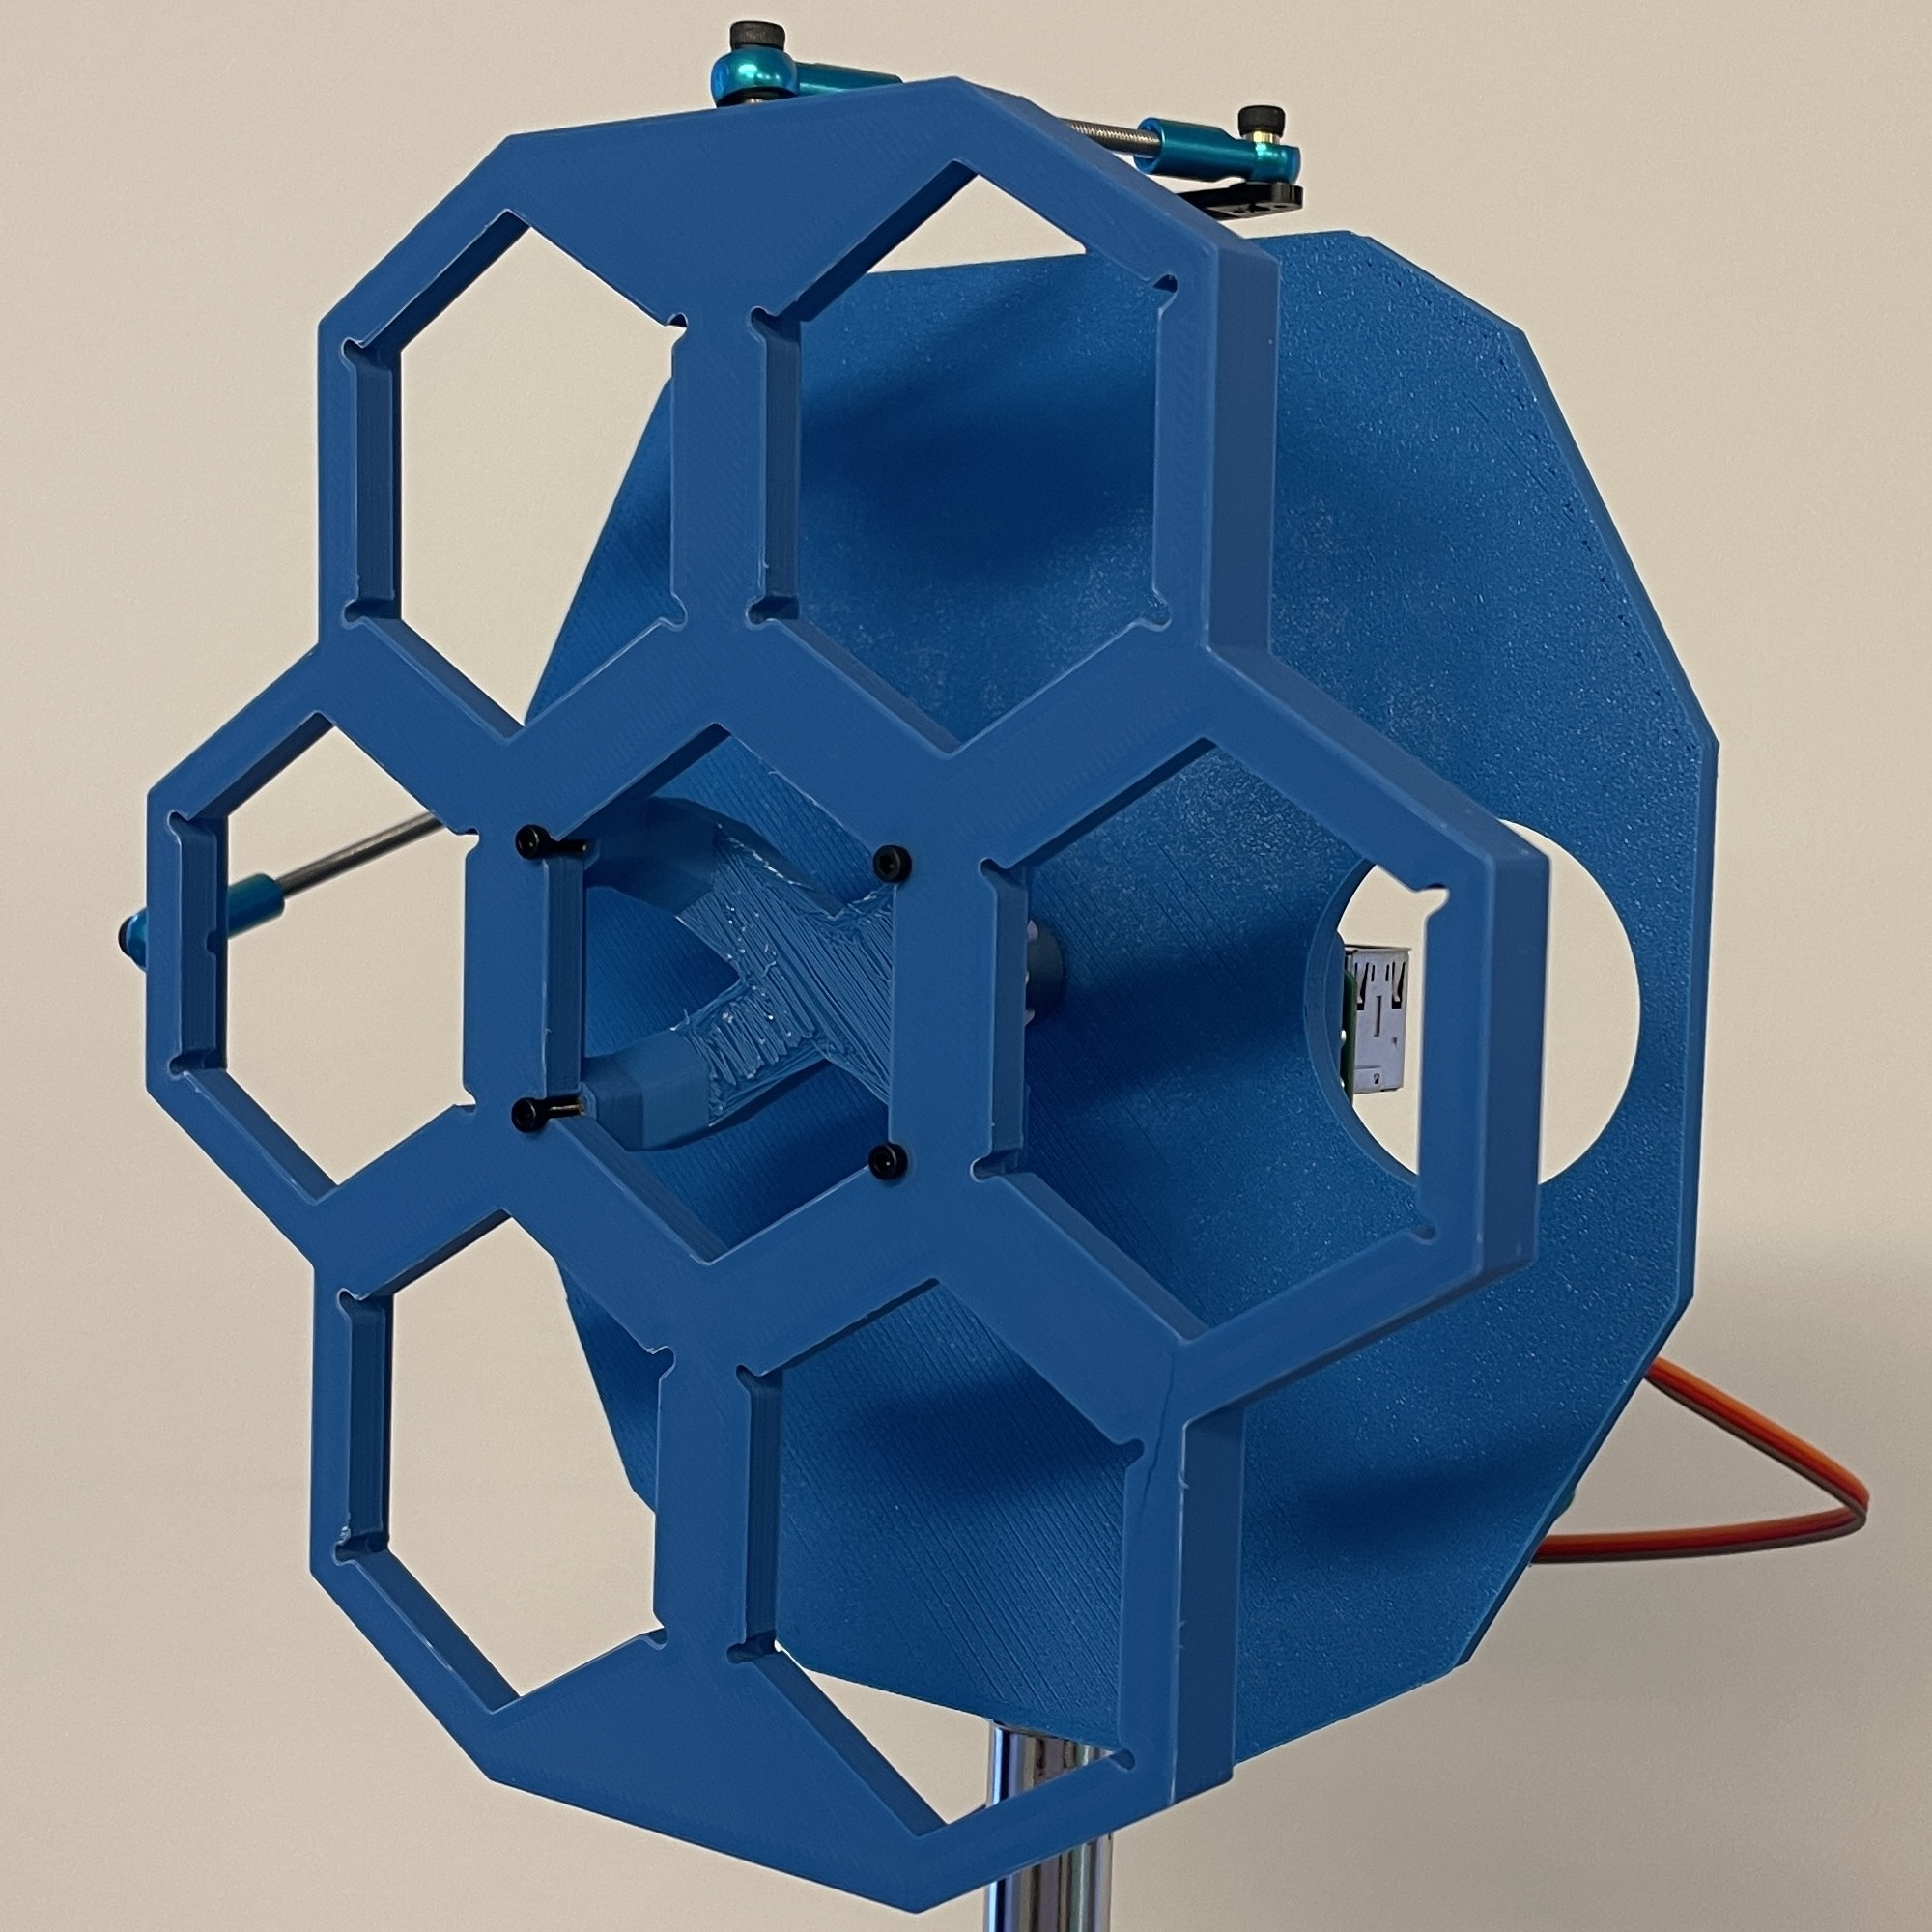
\includegraphics[width=\textwidth]{src/assets/pictures/construction/construction_front.JPG}
    \caption{Front view}
    \label{fig:const:int:const_front}
  \end{subfigure}
  \hfill
  \begin{subfigure}[b]{0.49\textwidth}
    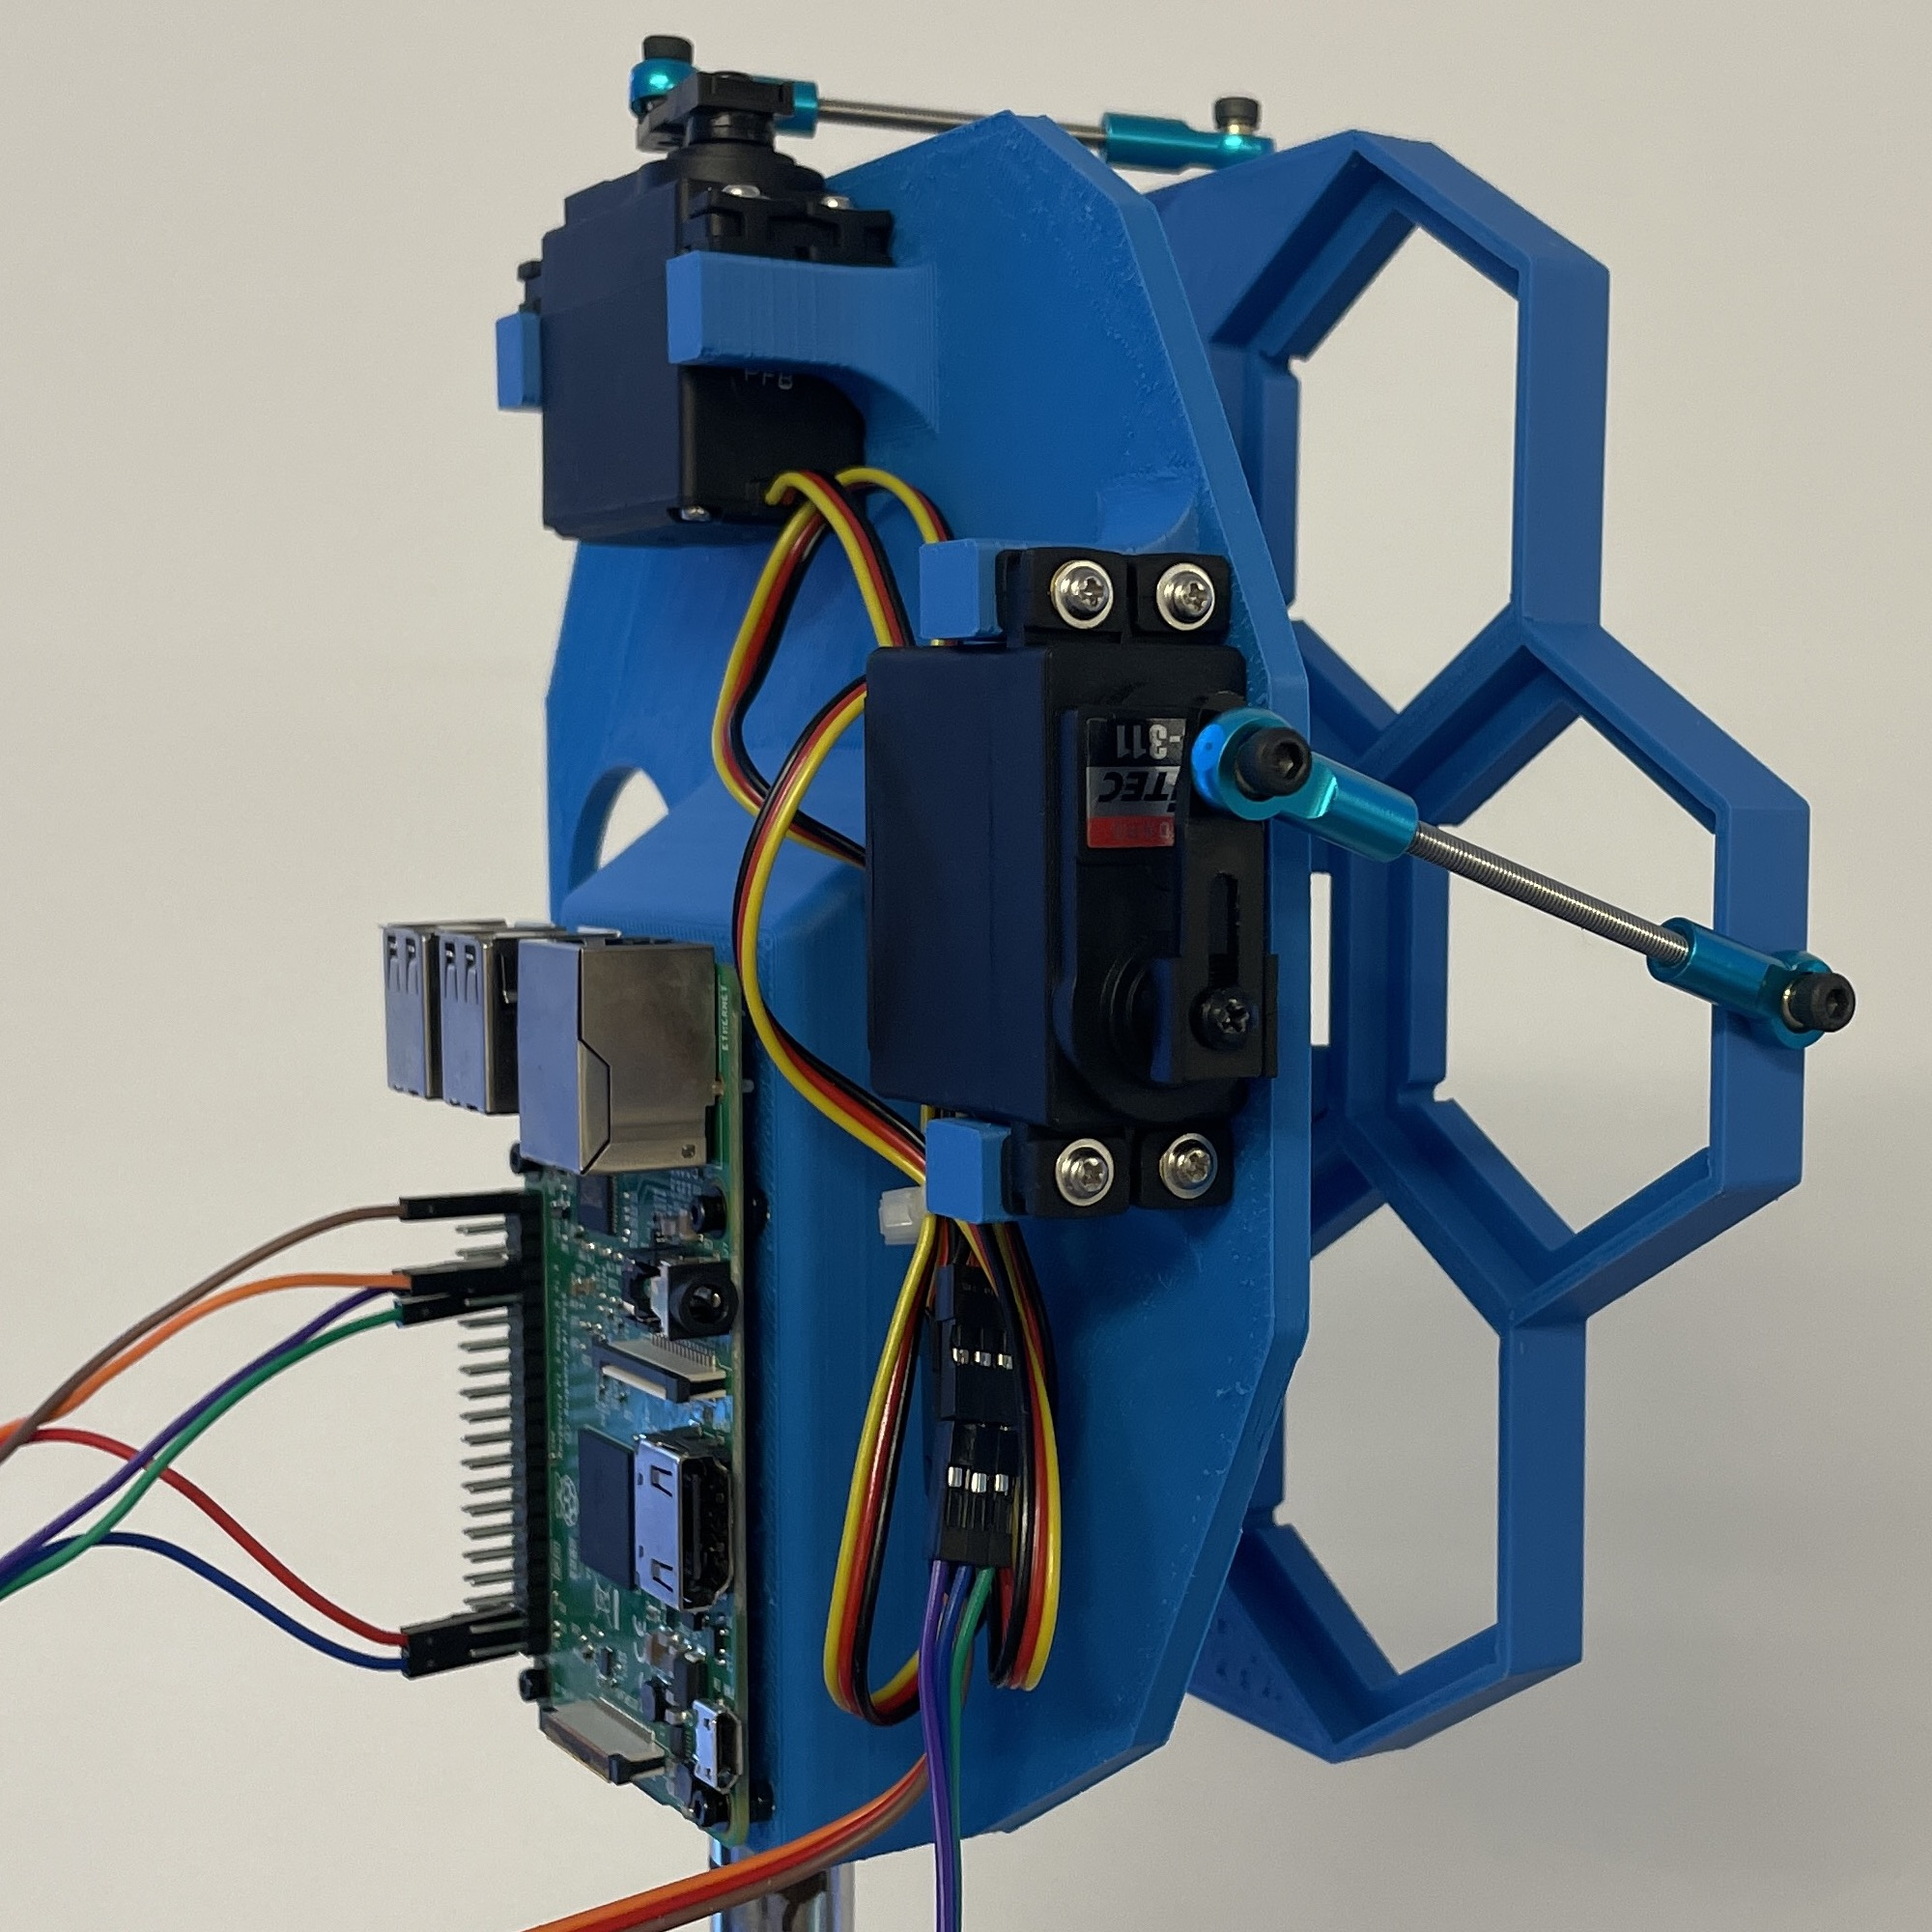
\includegraphics[width=\textwidth]{src/assets/pictures/construction/construction_back.JPG}
    \caption{Back view}
    \label{fig:const:int:const_back}
  \end{subfigure}
  \caption{Complete speaker}
  \label{fig:const:int:const}
\end{figure}
%
\subsubsection*{Tilting mechanism}

The tilting mechanism is realized using a cardan joint (Figure \ref{fig:const:int:cardan_joint}) as joint (\textbf{A}). The rotation of \textbf{F} is created with servos. The shafts \textbf{D} and \textbf{E} are built with a servo arm and threaded rod connected with ball joints (Figure \ref{fig:const:int:shaft}). The whole construction is displayed in figure \ref{fig:const:int:const}
%
\begin{figure}[ht]
  \begin{subfigure}[b]{0.174\textwidth}
    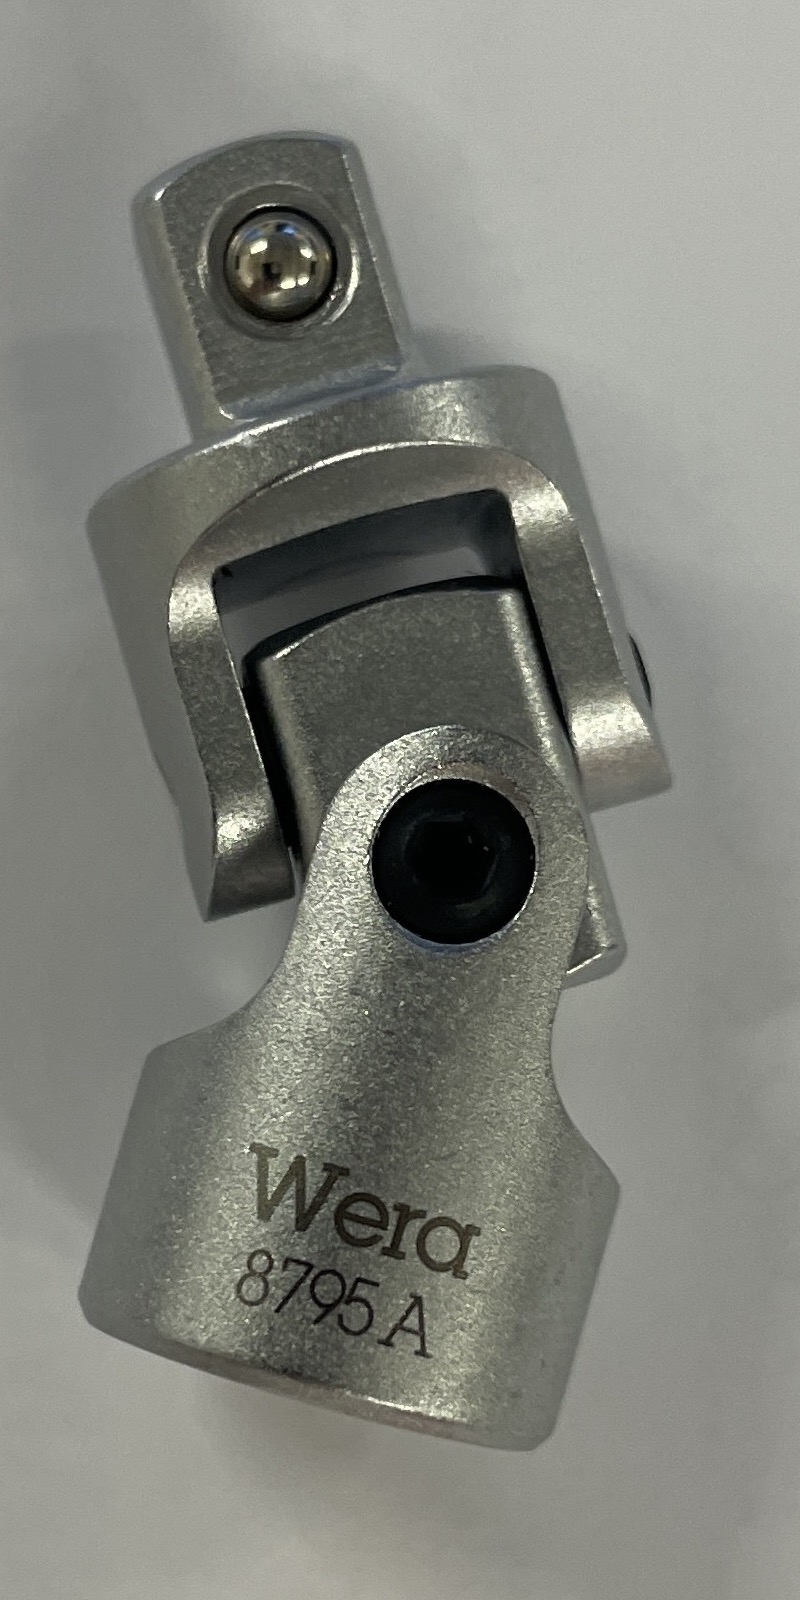
\includegraphics[width=\textwidth]{src/assets/pictures/construction/cardan_joint.JPG}
    \caption{Cardan Joint}
    \label{fig:const:int:cardan_joint}
  \end{subfigure}
  \hfill
  \begin{subfigure}[b]{0.80\textwidth}
    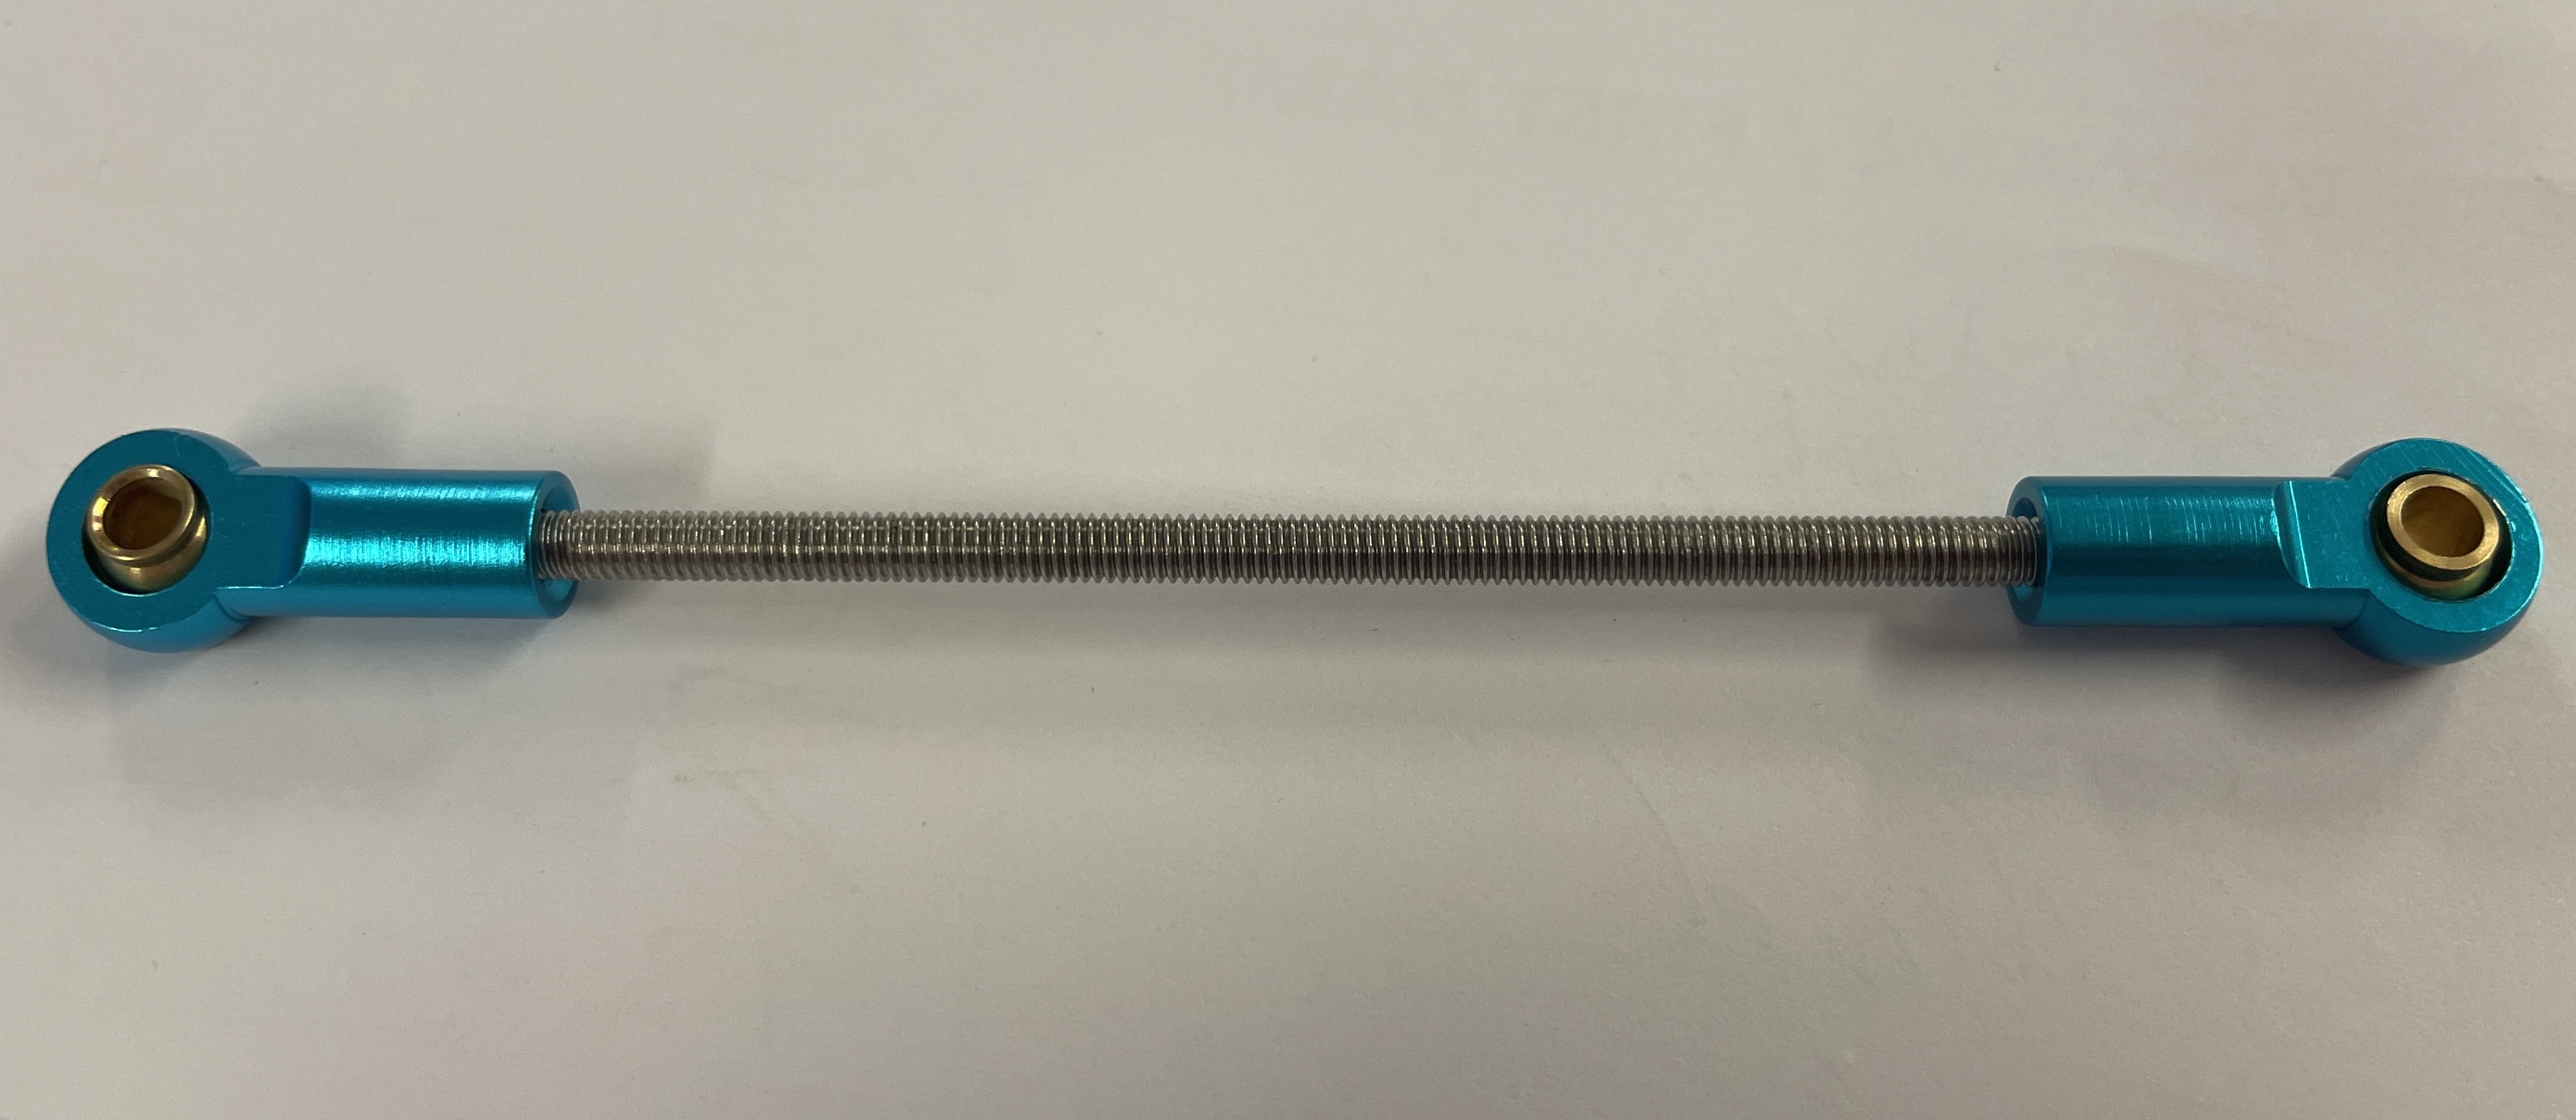
\includegraphics[width=\textwidth]{src/assets/pictures/construction/shaft.JPG}
    \caption{Shaft}
    \label{fig:const:int:shaft}
  \end{subfigure}
  \caption{Components for the tilting mechanism}
  \label{fig:const:int:tiltin_components}
\end{figure}
%
\subsubsection*{PCB mount}
%
One speaker module is mounted using a hexagon frame (Figure \ref{fig:const:int:mount}). The PCB can be screwed to this frame. To mount all modules, seven of those frames are combined to one model (Figure \ref{fig:const:int:const}). Screw holes on the top and the left side provide an option to attach the ball joints for the tilting mechanism. The cardan joint is connected using the model shown in figure \ref{fig:const:int:mount_back}. It is screwed to the back of the center PCB.
%
\begin{figure}[ht]
  \begin{subfigure}[b]{0.49\textwidth}
    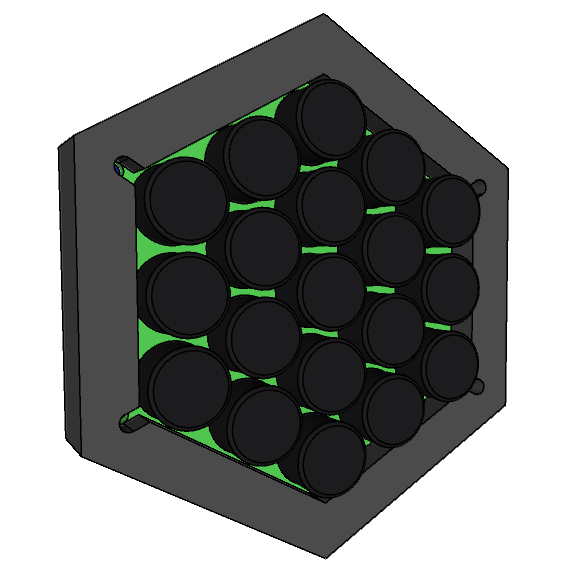
\includegraphics[width=\textwidth]{src/assets/pictures/construction/pcb_plate.png}
    \caption{Front view}
    \label{fig:const:int:mount_front}
  \end{subfigure}
  \hfill
  \begin{subfigure}[b]{0.49\textwidth}
    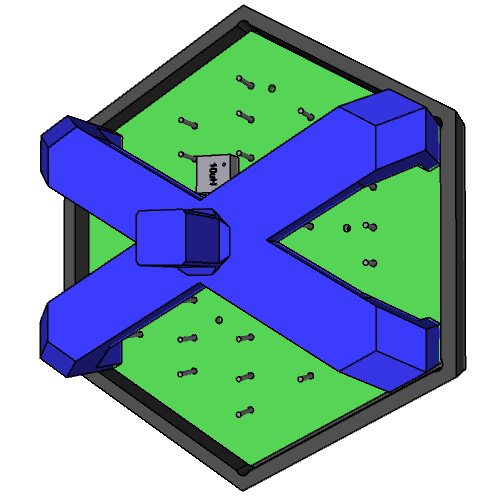
\includegraphics[width=\textwidth]{src/assets/pictures/construction/pcb_mount.png}
    \caption{Back view}
    \label{fig:const:int:mount_back}
  \end{subfigure}
  \caption{PCB mount model with cardan joint connector}
  \label{fig:const:int:mount}
\end{figure}
%
\subsubsection*{Base}

The base mimics the form of the PCB mount. A squared hole in the center allows the connection of the cardan joint. Servos are mounted to the back of the base at similar positions as the ball joints on the PCB mount. A thread on the bottom of the model will allow the speaker to be mounted on a tripod. The design of the base plate is shown in figure \ref{fig:const:int:base}.
%
\begin{figure}[ht]
  \begin{subfigure}[b]{0.48\textwidth}
    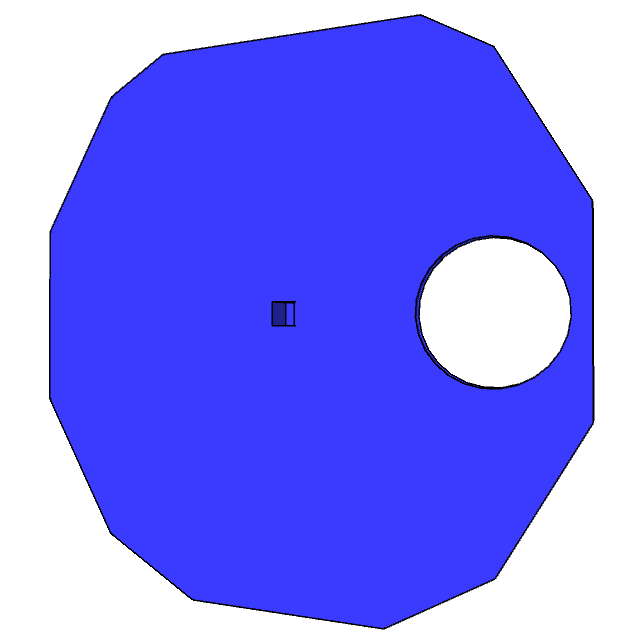
\includegraphics[width=\textwidth]{src/assets/pictures/construction/base_plate_front.png}
    \caption{Front view}
    \label{fig:const:int:base_front}
  \end{subfigure}
  \hfill
  \begin{subfigure}[b]{0.49\textwidth}
    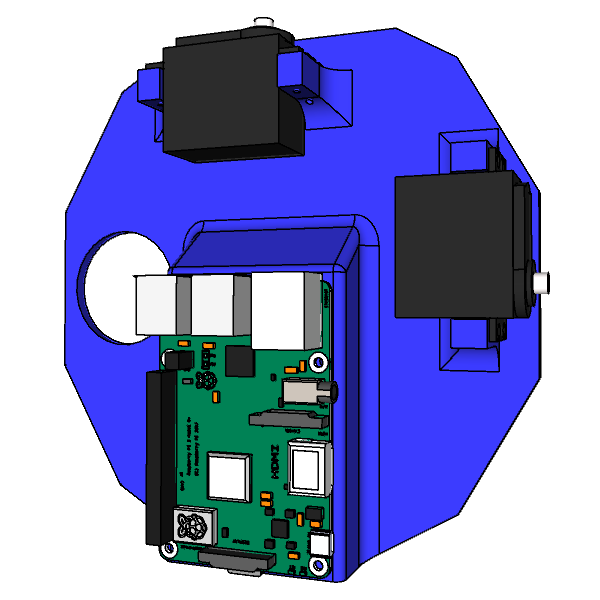
\includegraphics[width=\textwidth]{src/assets/pictures/construction/base_plate_back.png}
    \caption{Back view}
    \label{fig:const:int:base_back}
  \end{subfigure}
  \caption{Base plate model with servo motors and Respberry Pi}
  \label{fig:const:int:base}
\end{figure}